
\chapter{Arquitetura de Software}
\label{sec-arquitetura}
\vspace{-1cm}

A Figura~\ref{figura-arquitetura} mostra a arquitetura do sistema \emph{\imprimirtitulo}.

\begin{figure}[h]
	\centering
	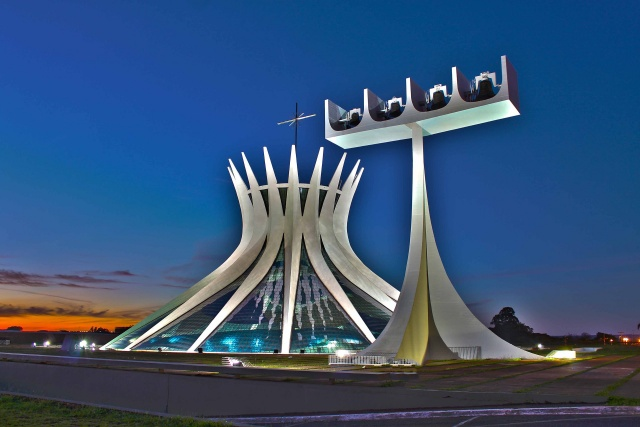
\includegraphics[width=0.8\textwidth]{figuras/figura-arquitetura}
	\caption{Arquitetura do sistema.}
	\label{figura-arquitetura}
\end{figure}

\vspace{0.5cm}

A arquitetura do sistema \emph{\imprimirtitulo} é baseada na Arquitetura em Camadas~\cite{tu2023layered}, adaptando a Arquitetura MVC~\cite{qureshi2014mvc}. Ela é composta por dois principais subsistemas, organizados em três camadas.
\begin{itemize}
	\item \textbf{Subsistema Controle Interno:} Responsável pelo gerenciamento interno do sistema, incluindo cadastro e manutenção de dados de funcionários, produtos, serviços e filiais.
	\item \textbf{Subsistema Atendimento Cliente:} Responsável pela interação com os clientes, abrangendo cadastro e login de clientes, agendamentos de serviços, histórico de atendimentos e registro de compras.
\end{itemize}
As camadas da arquitetura de cada subsistema são definidas como:
\begin{itemize}
	\item \textbf{Camada de Interface com o Usuário (CIU):} Responsável pela comunicação entre o usuário e o sistema, incluindo telas e controladores de interação.
	\item \textbf{Camada de Lógica de Negócio (CLN):} Implementa a lógica de aplicação e de domínio do problema. Aplica-se o padrão Camada de Serviço (Service Layer), separando a lógica de tarefas (CGT) da lógica de domínio (CDP).
	\item \textbf{Camada de Domínio do Problema (CDP):} Contém as classes que representam os conceitos e regras do domínio do problema.
	\item \textbf{Camada de Gerência de Dados (CGD):} Responsável pela persistência e recuperação de dados, seguindo o padrão Data Access Object (DAO).
\end{itemize}
A comunicação entre as camadas segue o padrão MVC, onde as páginas do front-end (CIU) chamam os adaptadores responsáveis pelas respostas via protocolo RESTful no back-end, acionando as classes controladoras (CIU), que interagem com as classes da camada de lógica de negócios (CLN) que, por sua vez, se comunicam com as classes do domínio do problema (CDP) e com as classes gerenciadoras de dados (CGD).

A comunicação entre CLN ocorre primeiro com a CGD ao invés de ocorrer com a CDP devido o mapeamento de entidades de domínio para modelos de tabelas no banco de dados, que é responsabilidade da CGD.
Contudo, a comunicação é feita através de interfaces, promovendo baixo acoplamento e facilitando a manutenção e evolução do sistema.

\vspace{0.5cm}
